\documentclass{article}

\usepackage{icml2026}
\usepackage{amsmath}
\usepackage{amssymb}
\usepackage{booktabs}
\usepackage{graphicx}
\usepackage{adjustbox}
\usepackage{hyperref}
\usepackage{url}
\usepackage{tikz}
\usepackage{enumitem}
\setlist[itemize]{topsep=1.5pt,itemsep=1.5pt,parsep=0pt,partopsep=0pt,leftmargin=*}
\setlist[enumerate]{topsep=1.5pt,itemsep=1.5pt,parsep=0pt,partopsep=0pt,leftmargin=*}
\setlength{\textfloatsep}{8pt plus 2pt minus 2pt}
\setlength{\floatsep}{6pt plus 2pt minus 2pt}
\setlength{\intextsep}{6pt plus 2pt minus 2pt}
\raggedbottom

\icmltitlerunning{SAGE-Mem: Write-Time Defense for Adversarial and Unreliable Multimodal Agent Memory}

\begin{document}

\twocolumn[
\icmltitle{SAGE-Mem: Write-Time Defense for Adversarial and\\Unreliable Multimodal Agent Memory}

\begin{icmlauthorlist}
\icmlauthor{Anonymous Author}{}
\end{icmlauthorlist}

\icmlaffiliation{}{Anonymous Institution}

\icmlkeywords{multimodal agents, memory safety, prompt injection, adversarial robustness}

\vskip 0.3in
]

\printAffiliationsAndNotice{}

\begin{abstract}
Persistent memory improves long-horizon behavior, but it also makes unsupported observations durable: once written, they can be retrieved, summarized, and reused long after the original interaction. We study \textbf{write-time defense} for multimodal memory and introduce \textbf{SAGE-Mem}, a memory layer with typed memory stores, guard-based admission, Bayesian source trust, anomaly-aware write filtering, dependence-aware belief promotion, provenance-aware retrieval, and an optional LLM-based fallback guard for borderline write decisions. We evaluate SAGE-Mem with lifecycle metrics on an adversarial-and-noisy multimodal extension of LoCoMo-10 that we construct for this paper, and on a browser overwrite benchmark derived from MM-BrowseComp; for the main LoCoMo and VPI runs, we additionally report external LLM-judge evaluation. On the LoCoMo extension, SAGE-Mem drives write admission and retrieval contamination to zero, but yields lower benign utility than a retrieval-time baseline, exposing an integrity--utility tradeoff. On MM-BrowseComp, a provenance prior alone is insufficient for browser-derived overwrite attacks, motivating \textbf{SAGE-Mem-BrowseGuard}, a browser-specific write policy that combines typed claim control with composite semantic suspicion scoring; BrowseGuard blocks all 388 overwrite attempts while preserving near-clean utility.
\end{abstract}

\section{Introduction}

Persistent memory changes the failure mode of an agent. A stateless model can only be manipulated within the current context window; a stateful agent can be manipulated by altering the memory that later reasoning depends on. Persistent memory is therefore a durable attack surface rather than just a transient prompt-level vulnerability~\cite{ref1,ref2,ref3}. The problem is sharper in multimodal settings, where OCR text, vision captions, browser outputs, and tool messages are not interchangeable evidence channels. A single adversarial image can generate both OCR text and a caption-like description, creating the appearance of corroboration even though both observations derive from the same corrupted source. Multimodal agreement can therefore reflect \emph{dependent corruption}, not independent evidence~\cite{ref8}.

Most existing defenses address this problem too late. Retrieval-time scoring and inference-time robustness methods can reduce the chance that a poisoned item is surfaced, but they do not restore the memory state once unsupported content has been admitted~\cite{ref4,ref5,ref6,ref7}. A permissive store creates three downstream costs: state corruption, repeated retrieval burden, and compounding distortion when later summaries, belief promotion, or consolidation steps inherit unsupported content. We therefore study \textbf{write-time governance}: the system should decide which observations are allowed to become persistent state before they can influence later retrieval, summarization, and consolidation.

Our claim is deliberately narrow. We do not attempt full multimodal truth inference. Instead, we ask when heterogeneous multimodal observations should become persistent state, when they should remain weak evidence, and when apparent cross-modal agreement should be discounted because it comes from the same source object. \textbf{Contributions.} \textbf{(1)} We introduce \textbf{SAGE-Mem}, a governed memory layer with guard-based admission, Bayesian source trust, anomaly-aware write filtering, typed memory stores, dependence-aware belief promotion, and an optional LLM-based fallback guard for borderline write decisions. \textbf{(2)} We construct an adversarial-and-noisy multimodal extension of LoCoMo and a browser overwrite benchmark derived from MM-BrowseComp. \textbf{(3)} We introduce lifecycle metrics that separate write admission, belief formation, retrieval contamination, and downstream utility, supplemented with external LLM-judge evaluation for the main LoCoMo and VPI runs.

\section{Method}

SAGE-Mem sits between heterogeneous observations and a downstream planner. All candidate writes first pass a semantic write boundary and enter typed memory stores for \emph{evidence}, \emph{belief}, and \emph{control}. The key design choice is that admitted evidence is not automatically durable belief: suspicious or conflicting writes are routed to audit, while only sufficiently supported and traceable claims are later promoted into answer-bearing belief memory (Figure~\ref{fig:scale-arch}).

For an observation \(o\) from channel \(c\) and source \(s\), admission is controlled by a conjunction of semantic, trust, and anomaly checks:
\begin{equation}
\begin{aligned}
\operatorname{acc}(o)=1 \iff\;& g_{\mathrm{sem}}(o)=\mathrm{DATA},\\
& \tilde{\theta}(c,s,o)\ge\tau_t,\ d_M(o)\le\xi_t,\\
& \neg \psi_{\mathrm{VPI}}(o),\ \neg u_{\mathrm{conf}}(o)
\end{aligned}
\end{equation}
where \(g_{\mathrm{sem}}(o)\) is a semantic write-time guard, \(\tilde{\theta}(c,s,o)\) is source-conditioned trust after source priors, per-channel Bayesian updates, and browser-specific trust caps, \(d_M(o)\) is a session anomaly score, and \(u_{\mathrm{conf}}(o)\) flags unsafe conflict with higher-trust memory.

In the implementation, \(g_{\mathrm{sem}}(o)\) combines lightweight procedural screening with an optional LLM semantic guard or skeptic--advocate ensemble that classifies each write as \texttt{DATA}, \texttt{DIRECTIVE}, or \texttt{METADATA}. \texttt{DIRECTIVE} or high-risk items are quarantined into audit memory, \texttt{METADATA} is dropped, and passed \texttt{DATA} can carry extracted atomic facts into evidence memory at write time.

For the reported paper runs, source priors are fixed from the threat model rather than learned from benchmark outcomes. The ordering is: authenticated user \(>\) internal tool output \(>\) OCR / vision caption \(>\) browser-derived text \(>\) self-summary \(>\) echoed content \(>\) attacker. At runtime these priors are refined by per-channel Bayesian trust updates and a reactive threshold that tightens after quarantine events. Browser-derived text also receives a lower trust cap than internal tool output, reflecting that page content is externally controlled.

Belief promotion is gated separately from write admission:
\begin{equation}
\begin{aligned}
\operatorname{prom}(q)=1 \iff\;& |P_{\tau_p}(q)|\ge k_s,\\
& |\operatorname{indep}(P_{\tau_p}(q))|\ge k_i,\\
& \neg \operatorname{conflict}(P(q))
\end{aligned}
\end{equation}
where \(P_{\tau_p}(q)\) denotes supporting evidence for candidate belief \(q\) above threshold \(\tau_p\).
This matters because OCR and caption outputs from the same image should not count as two independent votes for the same claim. In the implementation, promoted beliefs also require conflict-free support and, for visually anchored evidence, non-visual corroboration; unsupported belief items are not used for planning retrieval.

Overall, the architecture implements the following state transition:
\begin{equation}
\begin{aligned}
g_{\mathrm{sem}}(o) &=
\begin{cases}
G_{\mathrm{proc}}(o), & \text{if the write is easy to classify},\\
G_{\mathrm{LLM}}(o), & \text{if the write is borderline},
\end{cases}\\
\mathcal{M}_{t+1} &=
\begin{cases}
\mathcal{M}_t \cup \{\operatorname{audit}(o_t)\}, & \operatorname{acc}(o_t)=0,\\
\mathcal{W}\!\left(\mathcal{M}_t,\mathrm{facts}(o_t)\right), & \operatorname{acc}(o_t)=1,
\end{cases}
\end{aligned}
\end{equation}
where \(\mathcal{W}\) writes guarded evidence immediately and promotes only claims satisfying \(\operatorname{prom}(q)=1\). Planning then retrieves from \(\mathcal{M}_{t+1}\) with provenance-aware scoring, while the external LLM judge in Figure~\ref{fig:scale-arch} is evaluation-only.

MM-BrowseComp exposes a further failure mode: browser-mediated belief revision. We therefore introduce \textbf{SAGE-Mem-BrowseGuard}, a browser-specific write-time defense with two layers. First, a composite Adversarial Belief Revision scorer caps trust for suspicious browser text using memory conflict, page-local outlierness, corroboration deficit, and channel-history signals. Second, typed claim control prevents externally controlled browser pages from directly writing \texttt{qa\_answer} claims into durable answer-bearing memory: browser content may write evidence, but not privileged answers.

\begin{figure*}[t]
\centering
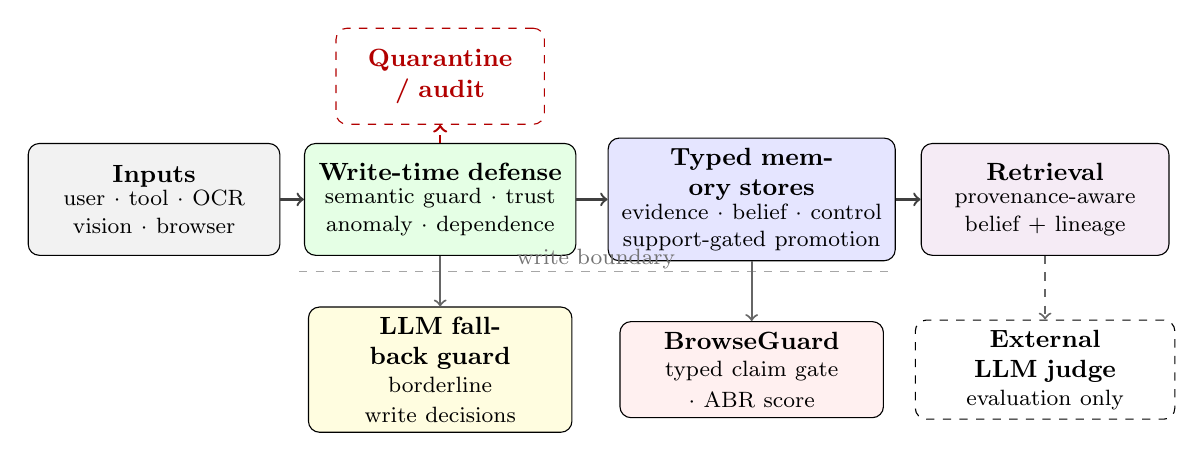
\begin{tikzpicture}[
  x=0.92cm,y=0.92cm,
  mainbox/.style={draw, rounded corners=4pt, align=center, font=\small, inner sep=3.5pt, minimum height=1.42cm, text width=2.95cm},
  subbox/.style={draw, rounded corners=4pt, align=center, font=\small, inner sep=3.5pt, minimum height=1.22cm, text width=3.1cm},
  evalbox/.style={draw, rounded corners=4pt, dashed, align=center, font=\small, inner sep=3.5pt, minimum height=1.22cm, text width=3.05cm},
  flow/.style={->, line width=0.85pt, draw=black!75},
  aux/.style={->, line width=0.75pt, draw=black!60},
  blocked/.style={->, dashed, line width=0.9pt, draw=red!70!black}
]
\node[mainbox, fill=gray!10] (src) at (0.0,0.0)
  {\textbf{Inputs}\\[-1pt]\footnotesize user $\cdot$ tool $\cdot$ OCR\\[-1pt]\footnotesize vision $\cdot$ browser};
\node[mainbox, fill=green!10, text width=3.2cm] (gate) at (3.95,0.0)
  {\textbf{Write-time defense}\\[-1pt]\footnotesize semantic guard $\cdot$ trust\\[-1pt]\footnotesize anomaly $\cdot$ dependence};
\node[mainbox, fill=blue!10, text width=3.4cm] (mem) at (8.25,0.0)
  {\textbf{Typed memory stores}\\[-1pt]\footnotesize evidence $\cdot$ belief $\cdot$ control\\[-1pt]\footnotesize support-gated promotion};
\node[mainbox, fill=violet!8, text width=2.9cm] (ret) at (12.3,0.0)
  {\textbf{Retrieval}\\[-1pt]\footnotesize provenance-aware\\[-1pt]\footnotesize belief + lineage};

\draw[flow] (src) -- (gate);
\draw[flow] (gate) -- (mem);
\draw[flow] (mem) -- (ret);

\draw[dashed, draw=black!35] (2.0,-1.0) -- (10.2,-1.0);
\node[font=\footnotesize, text=black!55] at (6.1,-0.82) {write boundary};

\node[subbox, fill=yellow!12] (llm) at (3.95,-2.35)
  {\textbf{LLM fallback guard}\\[-1pt]\footnotesize borderline write decisions};
\node[subbox, fill=red!6] (bg) at (8.25,-2.35)
  {\textbf{BrowseGuard}\\[-1pt]\footnotesize typed claim gate $\cdot$ ABR score};
\node[evalbox] (judge) at (12.3,-2.35)
  {\textbf{External LLM judge}\\[-1pt]\footnotesize evaluation only};
\node[evalbox, draw=red!70!black, text=red!70!black, text width=2.4cm] (quar) at (3.95,1.7)
  {\textbf{Quarantine / audit}};

\draw[aux] (gate.south) -- (llm.north);
\draw[aux] (mem.south) -- (bg.north);
\draw[aux, dashed] (ret.south) -- (judge.north);
\draw[blocked] (gate.north) -- (quar.south);
\end{tikzpicture}
\caption{SAGE-Mem architecture. A semantic write-time gate governs admission into typed memory stores for evidence, belief, and control; blocked writes are routed to quarantine before entering durable state. Borderline writes can be escalated to an LLM fallback guard, BrowseGuard adds browser-specific protection, and the dashed LLM-judge box is evaluation-only.}
\label{fig:scale-arch}
\end{figure*}

\section{Evaluation}

We evaluate in two regimes. First, we construct an adversarial-and-noisy multimodal extension of LoCoMo-10 by adding multimodal poisoning, Visual Prompt Injection (VPI), and noisy or missing-modality stressors. This extension is used specifically to test write admission, belief formation, and retrieval contamination under multimodal corruption. Second, we build a browsing-style benchmark from MM-BrowseComp observation traces with clean and adversarial tracks. The adversarial browsing benchmark contains 194 cases and injects two overwrite attempts per case: \texttt{fact\_overwrite\_injection} and \texttt{fact\_overwrite\_adaptive}. This lets us test whether a browsing defense is robust to paraphrased overwrite attacks rather than to one fixed wording.

Our primary metrics follow the memory lifecycle: \emph{attack write admission rate}, \emph{attack belief formation rate}, and \emph{retrieval contamination}. We also report \emph{BCU} (Benign Completion Under Attack), a joint metric that requires both answer consistency and attack suppression. For the LoCoMo main and VPI runs, we additionally use an external LLM judge for behavioral attack survival and answer entailment; the judge sees only retrieved context, the question, and the gold answer. Final-answer accuracy alone is insufficient for a memory defense whose main purpose is to keep unsupported content out of durable state.

\begin{table}[t]
\centering
\small
\setlength{\tabcolsep}{4.8pt}
\renewcommand{\arraystretch}{0.96}
\begin{adjustbox}{max width=\columnwidth}
\begin{tabular}{lrrr}
\toprule
Method & BCU poison & Write ASR & Retrieval ASR \\
\midrule
MMA & 0.6417 & 1.0000 & 0.1333 \\
RSum & 0.4533 & 0.0000 & 0.0067 \\
\textbf{SAGE-Mem} & \textbf{0.4600} & \textbf{0.0000} & \textbf{0.0000} \\
\bottomrule
\end{tabular}
\end{adjustbox}
\caption{Main LoCoMo result on the primary long-horizon benchmark. SAGE-Mem eliminates write admission and retrieval contamination, while MMA retains higher benign utility.}
\label{tab:locomo-main-3p}
\end{table}

\section{Results}

Table~\ref{tab:locomo-main-3p} establishes the central tradeoff in the paper. On LoCoMo, SAGE-Mem drives write admission and retrieval contamination to zero, whereas MMA preserves much higher utility by maintaining a broader memory store and filtering at retrieval time. The comparison is therefore not which method dominates overall, but which operating point is preferable: cleaner persistent state or higher short-term answer utility. This tradeoff is stable across seeds: SAGE-Mem achieves BCU$_{\text{poison}}=0.418\pm0.006$ with ASR \(=0.0\), while MMA achieves BCU$_{\text{poison}}=0.655\pm0.015$ with ASR \(=0.158\pm0.018\).

The multimodal evidence is consistent with the same story. On the VPI-only benchmark, SAGE-Mem suppresses both write admission and retrieval contamination to zero, supporting the claim that OCR and caption outputs from the same image should not be treated as independent corroboration. Under noisy or missing modalities, SAGE-Mem remains near-zero on retrieval contamination (Retrieval ASR \(=0.005\)), while the weaker H3 baseline degrades more substantially. The Bayes-style trust component matters primarily through calibration: it reduces over-quarantine under degraded multimodal evidence rather than changing the qualitative robustness story.

\begin{table}[t]
\centering
\small
\setlength{\tabcolsep}{4.6pt}
\renewcommand{\arraystretch}{0.96}
\begin{adjustbox}{max width=\columnwidth}
\begin{tabular}{lrrrr}
\toprule
Method & BCU clean & BCU poison & Write ASR & Retrieval ASR \\
\midrule
MMA & 0.1959 & 0.0000 & 1.0000 & 1.0000 \\
SAGE-Mem & 0.1649 & 0.2027 & 0.6521 & 0.5653 \\
SAGE-Mem-Browse & 0.1598 & 0.0189 & 0.6521 & 0.6907 \\
\textbf{BrowseGuard} & \textbf{0.1598} & \textbf{0.1546} & \textbf{0.0000} & \textbf{0.0000} \\
\bottomrule
\end{tabular}
\end{adjustbox}
\caption{MM-BrowseComp overwrite results (194 cases, 388 attack writes). BrowseGuard blocks overwrite without collapsing clean utility.}
\label{tab:mmbrowse-3p}
\end{table}

The browsing benchmark in Table~\ref{tab:mmbrowse-3p} sharpens the source-context story. A provenance prior alone is insufficient: \textbf{SAGE-Mem-Browse} is nearly identical to generic SAGE-Mem on write admission, showing that simply lowering trust for browser-originated text is too weak. By contrast, \textbf{BrowseGuard} blocks all 388 overwrite attempts and drives retrieval contamination to zero while preserving near-clean utility (BCU$_{\text{poison}}=0.1546$ vs.\ BCU$_{\text{clean}}=0.1598$). That is the relevant result for this workshop paper: browser-specific write control closes the overwrite path without sacrificing the operating point on clean browsing traces.

\section{Discussion}

Write-time governance is a useful robustness primitive for multimodal agent memory, but it should be evaluated as an integrity--utility tradeoff rather than as a universal replacement for retrieval-time filtering. On controlled long-horizon tasks, SAGE-Mem substantially improves memory-state integrity, including under VPI and noisy multimodal stress. On browsing tasks, source provenance alone is too weak; robust defense requires a browser-specific write policy that blocks browser-sourced factual assertions from entering answer-bearing memory directly. The main limits are equally clear: we assume trusted orchestration labels, the LoCoMo setting is controlled rather than fully naturalistic, and BrowseGuard's guarantee is specific to the evaluated overwrite threat model rather than all web-agent attacks.

\bibliography{references}
\bibliographystyle{icml2026}

\end{document}
